% $Header: /cvsroot/latex-beamer/latex-beamer/solutions/conference-talks/conference-ornate-20min.en.tex,v 1.7 2007/01/28 20:48:23 tantau Exp $

\documentclass{beamer}[10]

\usepackage{pgf}

\usepackage{handoutWithNotes}
\usepackage{pgfpages}
%\pgfpagesuselayout{3 on 1 with notes}[a4paper,border shrink=5mm] % Descomentar para presentacion con notas
\usepackage{movie15}

\definecolor{kugreen}{RGB}{50,93,61}
\definecolor{kugreenlys}{RGB}{132,158,139}
\definecolor{kugreenlyslys}{RGB}{173,190,177}
\definecolor{kugreenlyslyslys}{RGB}{214,223,216}
\setbeamercovered{transparent}
\mode<presentation>
\usetheme[numbers,totalnumber,compress,sidebarshades]{Lucas}
\setbeamertemplate{footline}[frame number]\usetheme[numbers,totalnumber,compress,sidebarshades]{Lucas}

 
%  \usecolortheme[named=kugreen]{structure}
  \usecolortheme{wolverineLucas}
 % \usecolortheme{dolphin}
  \useinnertheme{circles}
  \usefonttheme[onlymath]{serif}
  \setbeamercovered{transparent}
  \setbeamertemplate{blocks}[rounded][shadow=true]
 
%\logo{\includegraphics[width=1.5cm]{ugr}}
\title{Dynamic and Partially Connected Ring Topologies for Evolutionary Algorithms with Structured Populations}
\subtitle{A stigmergic presentation}
\author{C.M. Fernandes, \textbf{J.L.J. Laredo}, \textbf{J.J. Merelo}, C. Cotta, A. Rosa}
%\institute{University of Luxembourg}
\date{}

%\AtBeginSection[] % Do nothing for \section*
%{
%  \begin{frame}<beamer>
%    \frametitle{Outline}
%    \tableofcontents[currentsection]
%  \end{frame}
%}

%\AtBeginSubsection[] % Do nothing for \subsection*
%{
%  \begin{frame}<beamer>
%    \frametitle{Outline}
%    \tableofcontents[currentsection,currentsubsection]
%  \end{frame}
%}



% If you have a file called "university-logo-filename.xxx", where xxx
% is a graphic format that can be processed by latex or pdflatex,
% resp., then you can add a logo as follows:

% \pgfdeclareimage[height=0.5cm]{university-logo}{university-logo-filename}
% \logo{\pgfuseimage{university-logo}}



% Delete this, if you do not want the table of contents to pop up at
% the beginning of each subsection:
%\AtBeginSubsection[]
%{
%  \begin{frame}<beamer>{Outline}
%   \tableofcontents[currentsection,currentsubsection]
%  \end{frame}
%}


% If you wish to uncover everything in a step-wise fashion, uncomment
% the following command: 

%\beamerdefaultoverlayspecification{<+->}


\begin{document}

%%%%%%%%%%%%%%%%%%%%%%%%%%%%%%%%%%%%%%%%%%%%%%%%%%
\begin{frame}
  \titlepage
\end{frame}
%%%%%%%%%%%%%%%%%%%%%%%%%%%%%%%%%%%%%%%%%%%%%%%%%%
\note{Talk no more than 1 minute.}


%%%%%%%%%%%%%%%%%%%%%%%%%%%%%%%%%%%%%%%%%%%%%%%%%%
\begin{frame}{Outline}
  \tableofcontents
\end{frame}
%%%%%%%%%%%%%%%%%%%%%%%%%%%%%%%%%%%%%%%%%%%%%%%%%%
\note{Talk no more than 1 minute.}


%Juanlu: Incluyo algunos templates de diapositivas

\section{Introduction}

%%%%%%%%%%%%%%%%%%%%%%%%%%%%%%%%%%%%%%%%%%%%%%%%%%
\begin{frame}{What's the problem?}

%\begin{columns}

% \column{.5\textwidth}
%  \begin{itemize}
%   \item \textcolor{red}{Algorithm} %(a finite list of well-defined instructions for calculating a function)
%   \begin{itemize}
%    \item Calculus
%    \item Data processing
%    \item $\dots$
%   \end{itemize}
%  \item \textcolor{red}{Computational Intelligence}% (algorithms to solve complex real-world problems)
%  \begin{itemize}
%    \item Artificial neural-networks
%    \item Evolutionary computation
%    \item Swarm intelligence
%    \begin{itemize}
%      \item Particle swarm optimization
%      \item \textcolor{blue}{Ant colony optimization(ACO)}
%    \end{itemize}
%    \item $\dots$
%   \end{itemize}
%  \end{itemize}
% \column{.5\textwidth}

\begin{center} 
   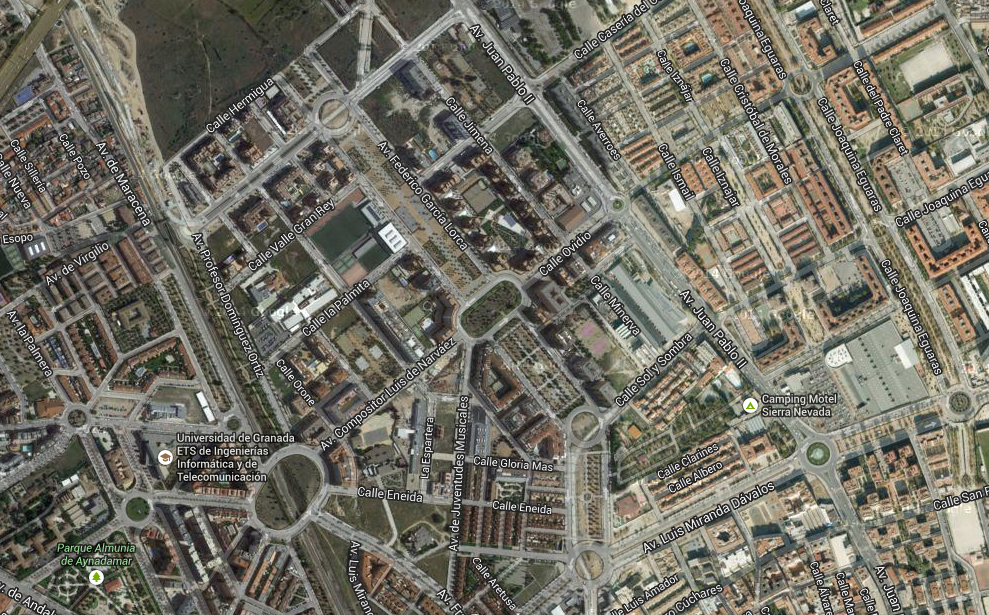
\includegraphics[width=0.9\textwidth]{images/citygrid.png} 
\end{center} 

%\end{columns}

\end{frame}
%%%%%%%%%%%%%%%%%%%%%%%%%%%%%%%%%%%%%%%%%%%%%%%%%%
\note{Talk no more than 1 minute.}

%%%%%%%%%%%%%%%%%%%%%%%%%%%%%%%%%%%%%%%%%%%%%%%%%%
\begin{frame}{Let's solve it!}

\begin{center} 
   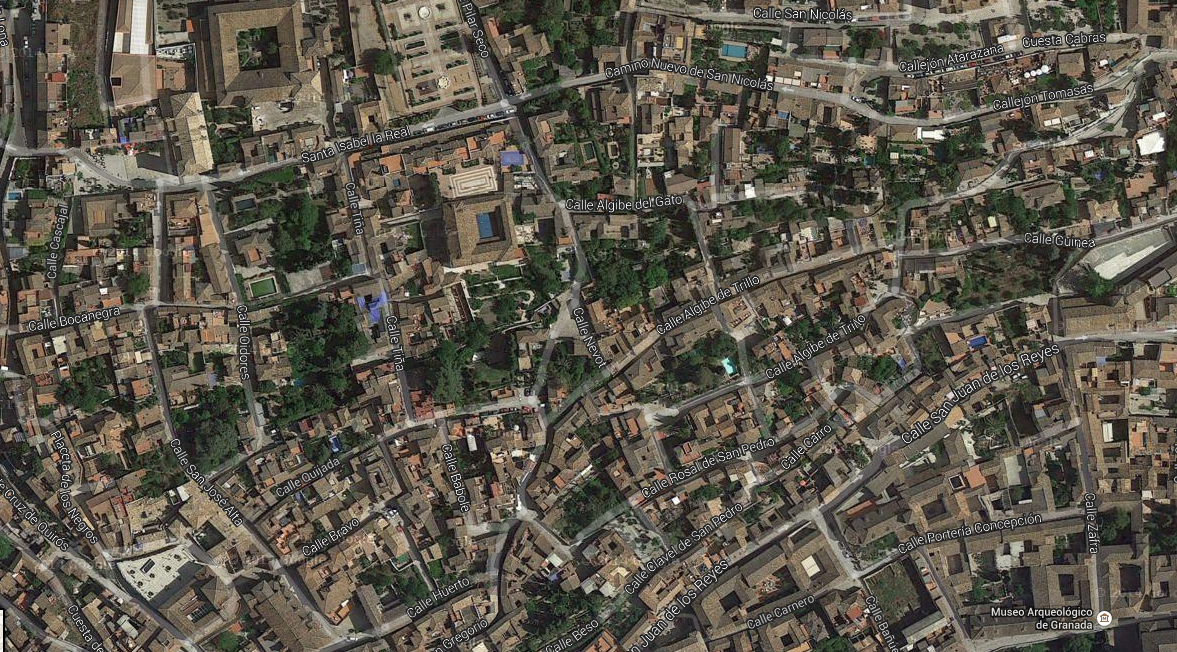
\includegraphics[width=0.9\textwidth]{images/albayzin.png} 
\end{center} 

%\end{columns}

\end{frame}
%%%%%%%%%%%%%%%%%%%%%%%%%%%%%%%%%%%%%%%%%%%%%%%%%%
\note{Talk no more than 1 minute.}


%%%%%%%%%%%%%%%%%%%%%%%%%%%%%%%%%%%%%%%%%%%%%%%%%%
\begin{frame}
\frametitle{A key concept: Emergence}
\begin{columns}
\column{.6\textwidth}
 \begin{itemize}
  \item Social animals like ants cooperate, which results in emergent behaviors
  \item<2-> But not only ants
 \end{itemize}
\column{.4\textwidth}
\includegraphics<1>[width=4cm]{images/al-Khwarizmi.png}
\includegraphics<2->[width=5cm]{images/geiser.png}
\end{columns}
\only<3>{
\begin{block}{Emergence [Wikipedia]}
Emergence is the way complex systems and patterns arise out of a multiplicity of relatively simple interactions.
\end{block}
}
\note{Picture from \url{https://www.flickr.com/photos/hdrphotographyblog/7831548420}}
\end{frame}
%%%%%%%%%%%%%%%%%%%%%%%%%%%%%%%%%%%%%%%%%%%%%%%%%%


 
%Juan Luis: Incluyo algunos templates de diapositivas

\section{Results at a glance}

%%%%%%%%%%%%%%%%%%%%%%%%%%%%%%%%%%%%%%%%%%%%%%%%%%
\begin{frame}{Gaps and clusters}

\begin{columns}
\column{.5\textwidth}
  \includegraphics<1>[width=5cm]{images/jambywaldec.png} 
  \includegraphics<2>[width=5cm]{images/spacediagram.png}

\column{.5\textwidth}
  
  \begin{itemize}
  \item DPTC dynamics resemblance traffic jams 
  \item Gaps and clusters form spontaneously
  \begin{itemize}
  	\item<2> $\frac{n}{Y}$ (Density)
  	\item<2> Movement criterion 
    \begin{itemize}
  		\item<2> Phenotype
  		\item<2> Genotype 
  		\item<2> Random 
    \end{itemize}  	
  	\item<2>  Cellular-Island Hybrid!? 
  \end{itemize}  
  \end{itemize}

\end{columns}

\end{frame}
%%%%%%%%%%%%%%%%%%%%%%%%%%%%%%%%%%%%%%%%%%%%%%%%%%
\note{Talk no more than 1 minute.}

%%%%%%%%%%%%%%%%%%%%%%%%%%%%%%%%%%%%%%%%%%%%%%%%%%
\begin{frame}{Results using trap functions}


\begin{columns}
\column{.75\textwidth}
\begin{scriptsize}
\begin{block}{Settings}
 \begin{itemize}
 \item $n=400$
 \item 2-trap $l=500$ 
 \item 3-trap $l=375$ 
 \item 4-trap $l=300$
 \item Top. (torus) (ring) (DPCT)
 \end{itemize}
\end{block}
\end{scriptsize}
\column{.25\textwidth}
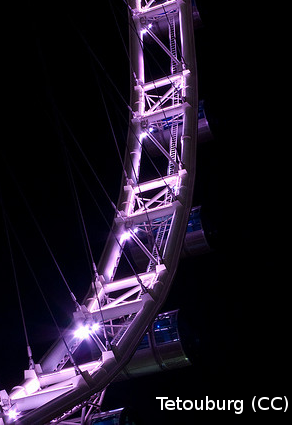
\includegraphics[width=2cm]{images/ringteutoburg.png} 
\end{columns}

\centering
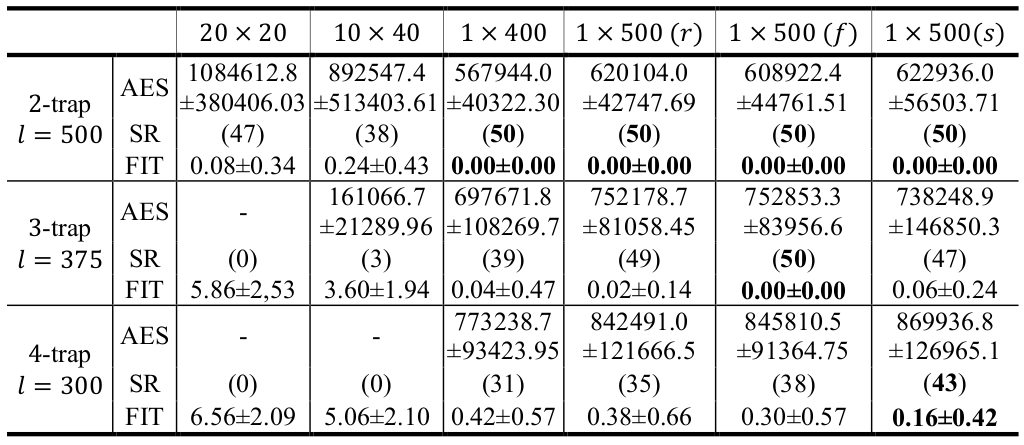
\includegraphics[width=9cm]{images/results1.png} 

\end{frame}
%%%%%%%%%%%%%%%%%%%%%%%%%%%%%%%%%%%%%%%%%%%%%%%%%%
\note{Talk no more than 1 minute.}

%%%%%%%%%%%%%%%%%%%%%%%%%%%%%%%%%%%%%%%%%%%%%%%%%%
\begin{frame}{Influence of density}
\begin{columns}
\column{.75\textwidth}
\begin{scriptsize}
\begin{block}{Settings}
 \begin{itemize}
 \item $n=400$
 \item 4-trap $l=300$
 \end{itemize}
\end{block}
\end{scriptsize}
\column{.25\textwidth}
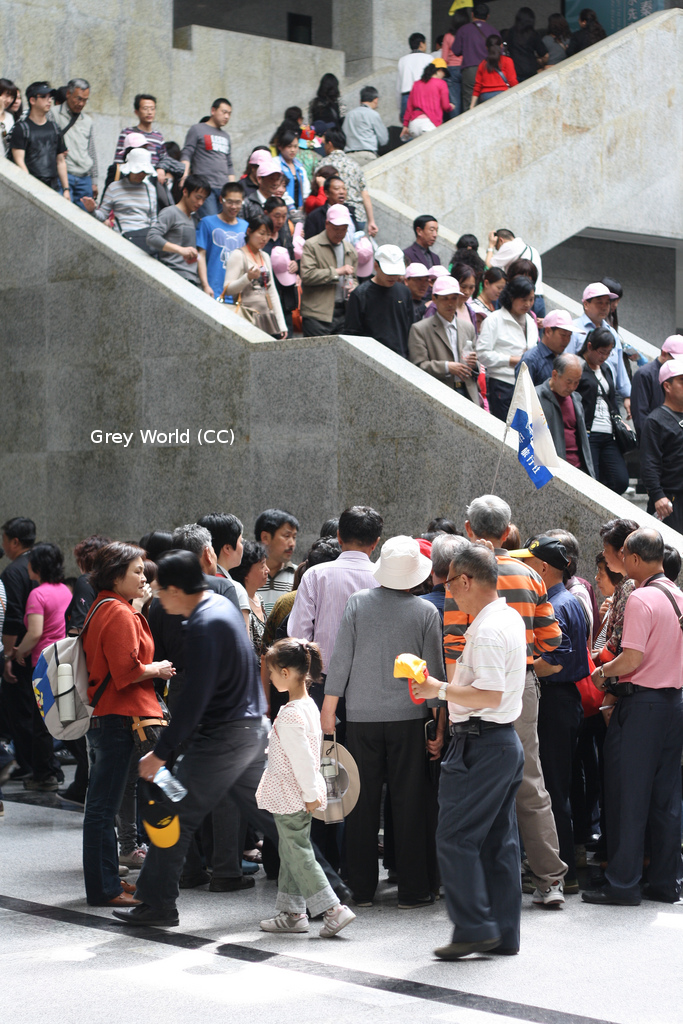
\includegraphics[width=2cm]{images/crowd.png} 

\end{columns}
\centering
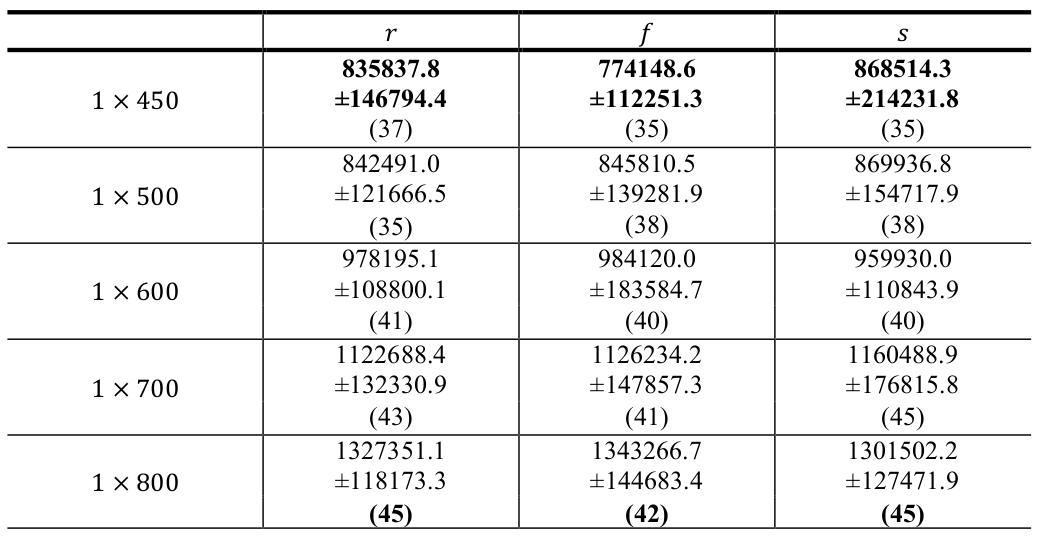
\includegraphics[width=8cm]{images/results2.png} 


\end{frame}
%%%%%%%%%%%%%%%%%%%%%%%%%%%%%%%%%%%%%%%%%%%%%%%%%%
\note{Talk no more than 1 minute.}


%%%%%%%%%%%%%%%%%%%%%%%%%%%%%%%%%%%%%%%%%%%%%%%%%%
\begin{frame}{What about optimal population sizes?}
\begin{columns}
\column{.75\textwidth}
\begin{scriptsize}
\begin{block}{Settings}
 \begin{itemize}
 \item \textst{n=400} $\rightarrow optimal$
 \item 4-trap 
 \end{itemize}
\end{block}
\end{scriptsize}
\column{.25\textwidth}
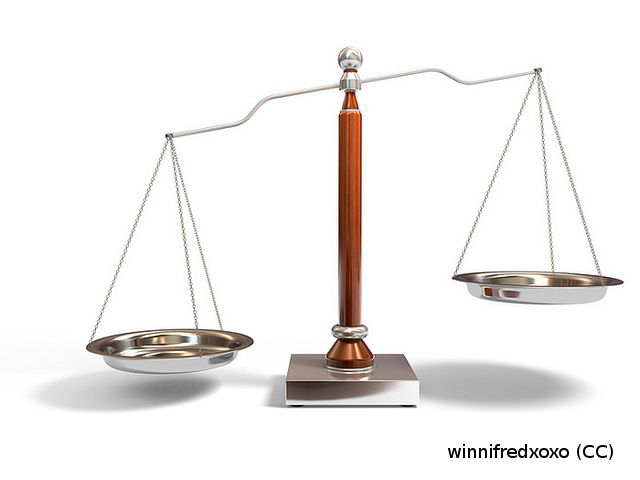
\includegraphics[width=2.5cm]{images/scale.png} 

\end{columns}
\centering
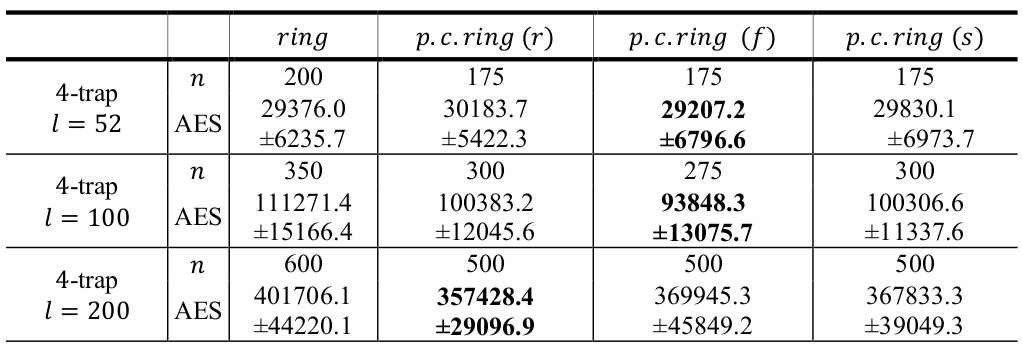
\includegraphics[width=10cm]{images/results3.png} 


\end{frame}
%%%%%%%%%%%%%%%%%%%%%%%%%%%%%%%%%%%%%%%%%%%%%%%%%%
\note{Talk no more than 1 minute.}



\section{Conclusions}

%%%%%%%%%%%%%%%%%%%%%%%%%%%%%%%%%%%%%%%%%%%%%%%%%%
\begin{frame}
\frametitle{Conclusions}

\begin{itemize}
\item Partially connected 1-dimensional cellular GA
\item The resulting structure displays an island-model behaviour 
\item Promotion of genetic diversity and reduction of the minimum population size
\end{itemize}

\only<2>{
\begin{block}{Future works}
 \begin{itemize}
 \item Extension to 2-dimensional model
 \item Modelling the DPCT in a probability-based model
 \end{itemize}
\end{block}
}
\end{frame}
%%%%%%%%%%%%%%%%%%%%%%%%%%%%%%%%%%%%%%%%%%%%%%%%%%



%-------------------------------------------------
%%%%%%%%%%%%%%%%%%%%%%%%%%%%%%%%%%%%%%%%%%%%%%%%%%
\begin{frame}{Questions?}
Thanks for your attention! 

Follow us at http://anyself.wordpress.com @geneura
\end{frame}
%%%%%%%%%%%%%%%%%%%%%%%%%%%%%%%%%%%%%%%%%%%%%%%%%%

\end{document}


